\chapter{Development of the Graph Language} \label{Concept_and_Implementation_of_the_Graph_Language}
In this chapter the concept and implementation of the graphical DSL tool is presented. First, the requirements for the editor are defined, and a suitable data structure with associations and attributes is designed, based on the foundations in Sect. \ref{Sequentially_Constructive_Statecharts}. Subsequently, the MGL is implemented, which uses the designed data structure as a basis. In addition, a style is created in the SGL for each component in the MGL, which defines the appearance of the element in the editor. After that, plug-ins for a better user interface are implemented. Finally, the realization of the code generator is presented, which can generate Java or C code from the created SCCharts models.

\section{Requirements}\label{Requirements}
Before the actual design process of the DSL tool can begin, it is essential to specify the main task and individual requirements, which are elaborated in more detail based on the problem statement.

The following main task results from the problem statement: The development of a graphical DSL tool for creating models of the visual modeling language SCCharts.
To further refine this task, requirements are established. These requirements are derived from considerations of the desired features of the editor. 

The developed tool or editor should be usable for creating models in the SCCharts language. The user interface should be as intuitive as possible, enabling domain experts without programming experience to create models. This means that it should be clear how to create a model, how to adjust and expand existing models, etc.. The editor should provide a palette of modeling elements that align with the specific requirements of the DSL. Therefore, a suitable data structure needs to be identified which can accurately represent the elements of the SCCharts language that are to be modulated. This includes properties or attributes that the components of the SCCharts language possess. Furthermore, the modeling elements should closely adhere to the visual syntax of SCCharts, making it clear which component in the SCCharts language the created element in the editor represents. Additionally, the editor should offer validation functions to ensure that the created models conform to the syntax of the DSL. Errors or inconsistencies should be reported to the user within the editor. A final central feature is that the user should have the ability to generate code in a target language such as Java or C from the created model, which can be utilized to be integrated in software projects. This requires a clear mapping of modeling elements to code constructs.
This results in five core requirements in addition to central ones:
\begin{enumerate}
\item The user interface is intuitive and easy to understand.
\item The underlying data structure correctly represents important relationships and attributes.
\item The visual syntax allow clear identification of the individual components of the SCCharts language.
\item Errors in models are indicated by validation with in the editor.
\item The editor provides code generation from designed models to integrable Java or C code.
\end{enumerate}
Based on these core requirements, designs are now being created to facilitate subsequent implementation.

\section{Data Structure}\label{Data Structure}
A decisive factor in the model transformation is the data structure. This must contain all relevant attributes and associations to adequately represent the elements of the SCCharts language. The correct design of this data structure is of fundamental importance, as it forms the basis for the entire modeling and transformation. First, the individual elements of SCCharts to be implemented within the framework of the editor are examined in more detail, then the relationship between them is examined.

\subsection{Model Elements}
Fig. \ref{fig:Component_Classes} shows all elements of the data structure as classes and subclasses that shall be implemented in the MGL. 
\begin{figure}[h!]
\centering
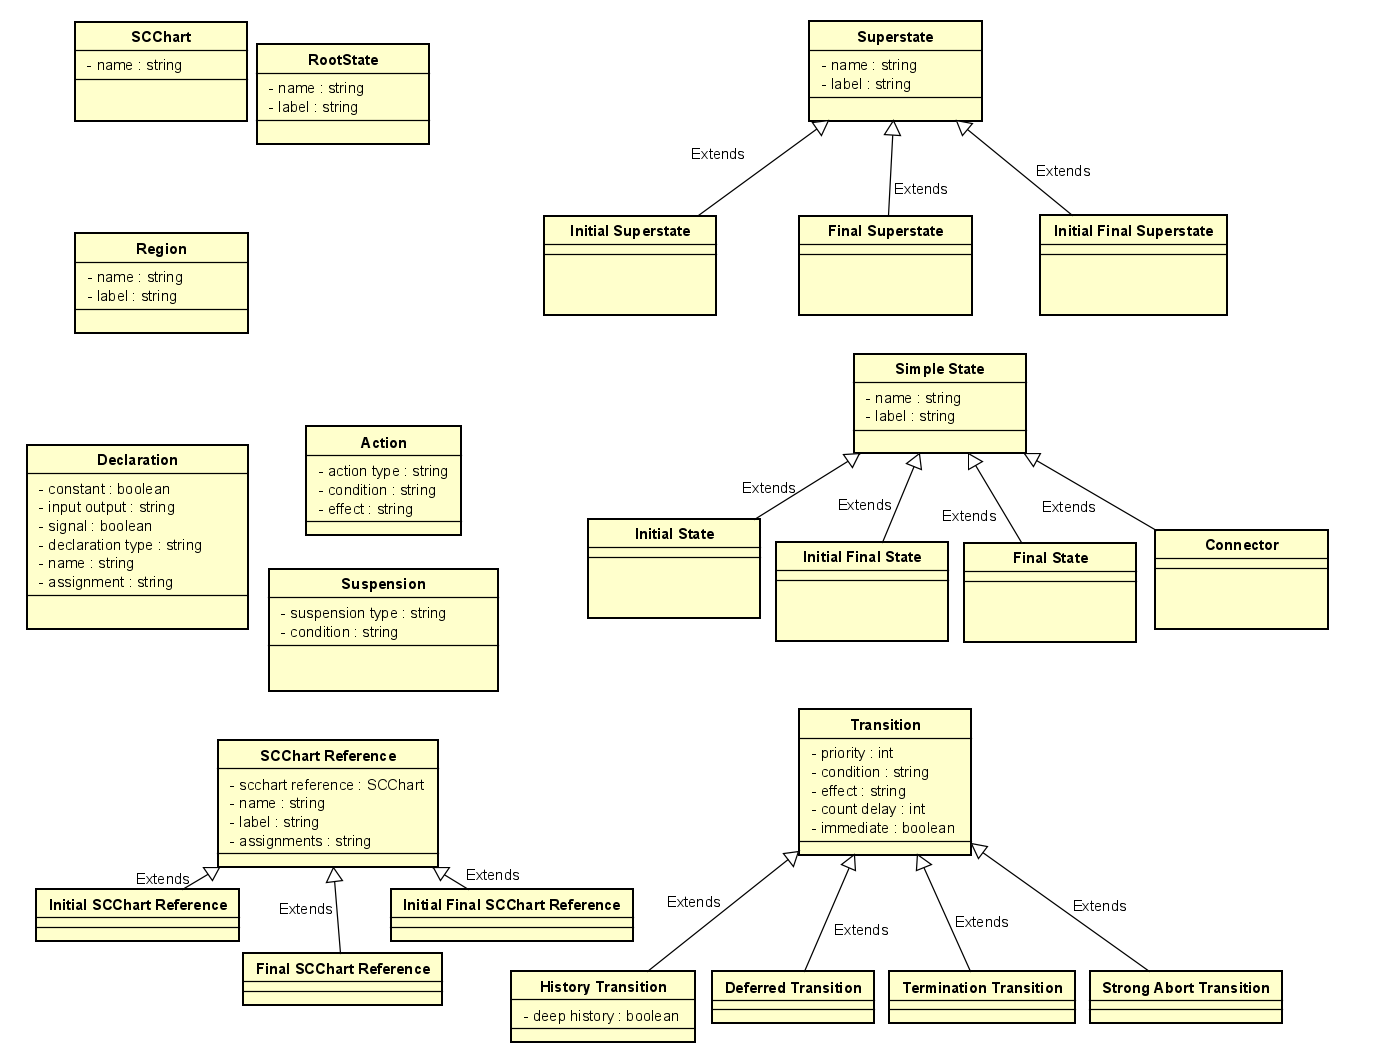
\includegraphics[width=1.0\textwidth]{bilder/Component_Classes.png}
\caption{Classes of the individual components}
\label{fig:Component_Classes}
\end{figure} 
\subsubsection{SCChart, Root State and Region}
The basis is the SCChart model itself, which must have a unique name in form of a string and no other attributes. In addition, there is the root state, of which exactly one exists and which must also have a unique name. Optionally, a label can be added that is displayed as a name when it is set. The same applies to regions, with the exception that here both the name and the label are optional. 
\subsubsection{Superstate and Simple State}
Superstates and simple states are additionally extended by initial, final and initial final states. In the case of simple states, additional connectors are added in the form of a subclass. Each of these states has an individual name and optionally a label, similar to the previously described root state classes.
\subsubsection{Declaration, Action and Suspension}
Declarations can occur on the one hand as constants or signals, which is represented by a boolean value. In addition, they can be declared as input, output, input output or local variable (i.e. none of them). This is made possible by the string data type, as there are more than two options. In addition, they have a name, a declaration type (for datatype) and optionally an assignment, all three of which are represented as strings. Actions and suspensions each have a type and a condition (also known as a trigger), which are defined as strings. In addition, actions have an effect, which is also a string.
\subsubsection{Transition}
Transitions have a priority and a count delay, both of which are represented as integers. In addition, they have a condition (trigger) and an effect (action), which are represented as strings. Furthermore, it is specified whether they are immediate or delayed, whereby this is represented with a boolean value.

The transition class is extended by four subclasses: history transition, deferred transition, termination transition and strong abort transition. The history transition also has a boolean attribute that is used to display deep or shallow history.

In addition to the transition subclasses mentioned, there are other combinations of transition types that are made up of the transition subclasses. An example would be a history transition that is also deferred, i.e. a deferred history transition. This results in a total of twelve different possible transitions. Namely: \textit{transition}, \textit{termination transition}, \textit{strong abort transition}, \textit{deferred transition}, \textit{history transition}, \textit{deferred termination transition}, \textit{deferred strong abort transition}, \textit{termination history transition}, \textit{strong abort history transition}, \textit{deferred history transition}, \textit{deferred strong abort history transition} and \textit{deferred termination history transition}.
\subsubsection{SCChart Reference}
The last component of the data structure is the SCChart reference class. Similar to the superstate class, it has subclasses including initial, final, initial final SCChart references, along with same attributes of the superstate class. Furthermore, it contains a SCChart reference with a SCChart type, and assignments in the form of strings that are necessary for the inputs and outputs of the referenced SCChart.

\subsection{Model Elements Associations and Relations}
Now that the individual components of the data structure have been defined, the relationships and associations between them can be considered. Fig. \ref{fig:ClassDiagramAssociation} represents the class diagram of the data structure that is to serve as the basis for the SCCharts model editor. All associations between the components are illustrated. The fundamental element for this diagram is the SCChart class, which serves as the root element for all other elements. 

The SCChart class contains exactly one root state, which, in turn, contains at least one region and can have an arbitrary number of declarations, suspensions, and actions. Within regions, there can be an arbitrary number of simple states or their subclasses, from which any number of transitions can originate and enter. Furthermore, regions can contain multiple superstates, each of which can have an arbitrary number of regions, declarations, suspensions, and actions. Additionally, an arbitrary number of transitions can connect these elements with others. Lastly, regions can contain any amount of SCChart references, which can, in turn, be linked with an arbitrary number of transitions. Additionally, these SCChart references reference one SCChart.

The created data structure can now be used for the model transformation.
\begin{figure}[h!]
\centering
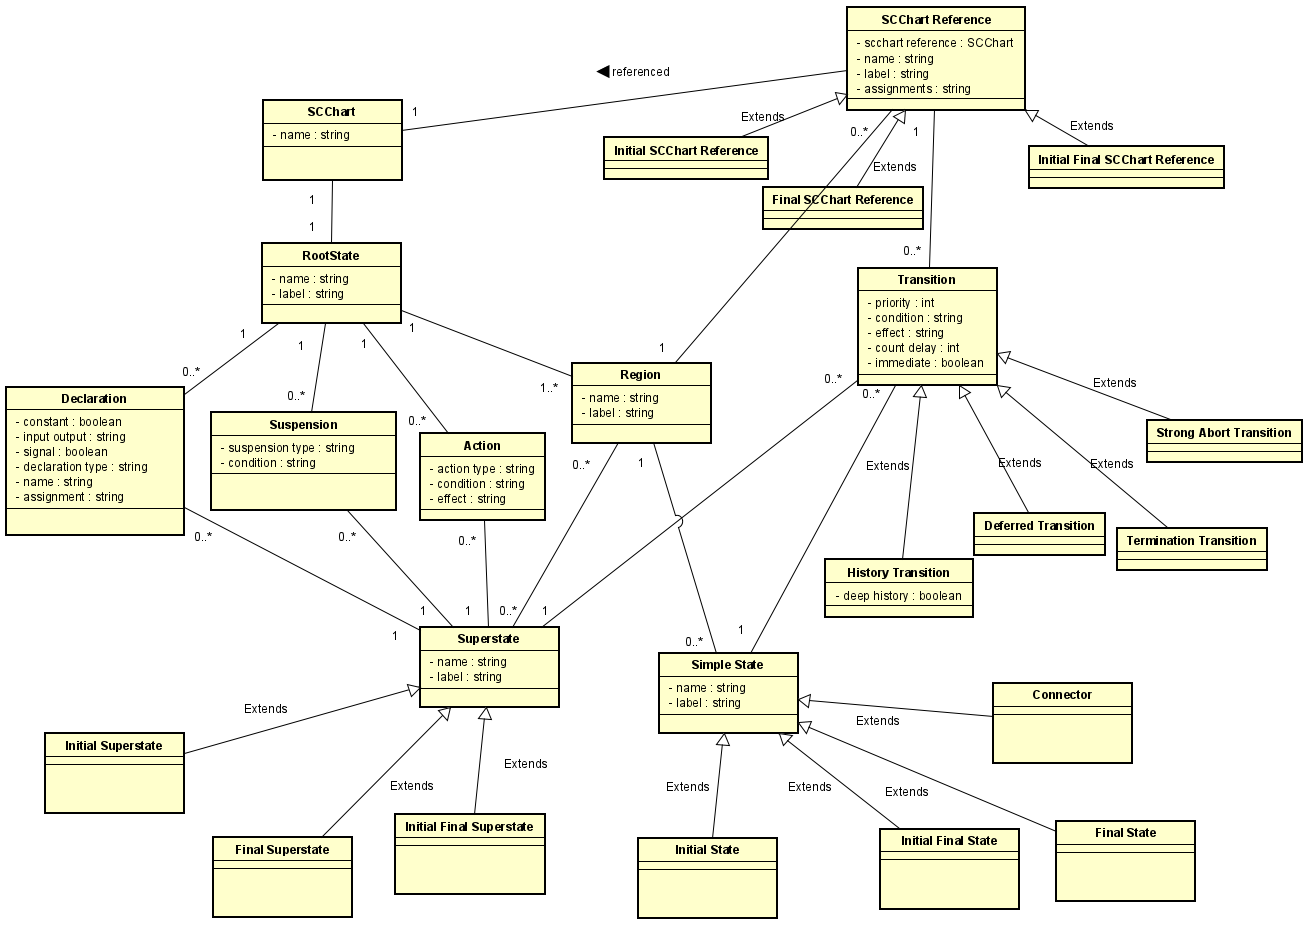
\includegraphics[width=1.0\textwidth]{bilder/ClassDiagramAssociation.png}
\caption{The class diagram of the designed data structure}
\label{fig:ClassDiagramAssociation}
\end{figure} 
\section{Model Transformation}
The model transformation of each \textsc{Cinco} Product is based on the MGL and the MSL, in which all components and their visual representation are defined. In addition to the graph model, the MGL consists of further components of the type node, edge, container. The elements of the designed data structure have to be mapped to the types of the meta graph model of \textsc{Cinco} for the implementation of the MGL. It is crucial to determine which component of the data structure can best be represented by which type of the \textsc{Cinco} meta graph model. 

In Fig. \ref{fig:MappingModelTransformation}, the meta graph model types of \textsc{Cinco} were mapped to the designed SCChart data structure. The class diagram of \textsc{Cinco}'s meta graph model elements can be seen at the top left, with the components graph model (blue), container (green), node (red) and edge (yellow). Below this is the designed SCChart data structure, whose classes have been colour-coded according to \textsc{Cinco}'s meta graph model elements. The graph model was assigned to the SCChart class. All components with inner behaviour, i.e. those that can contain further containers and nodes, are elements of the type container. These include root state, region, superstate and SCChart references. Declaration, suspension, action and simple states, on the other hand, are components of the node type. Transitions were assigned accordingly as edges.

\begin{figure}[h!]
\centering
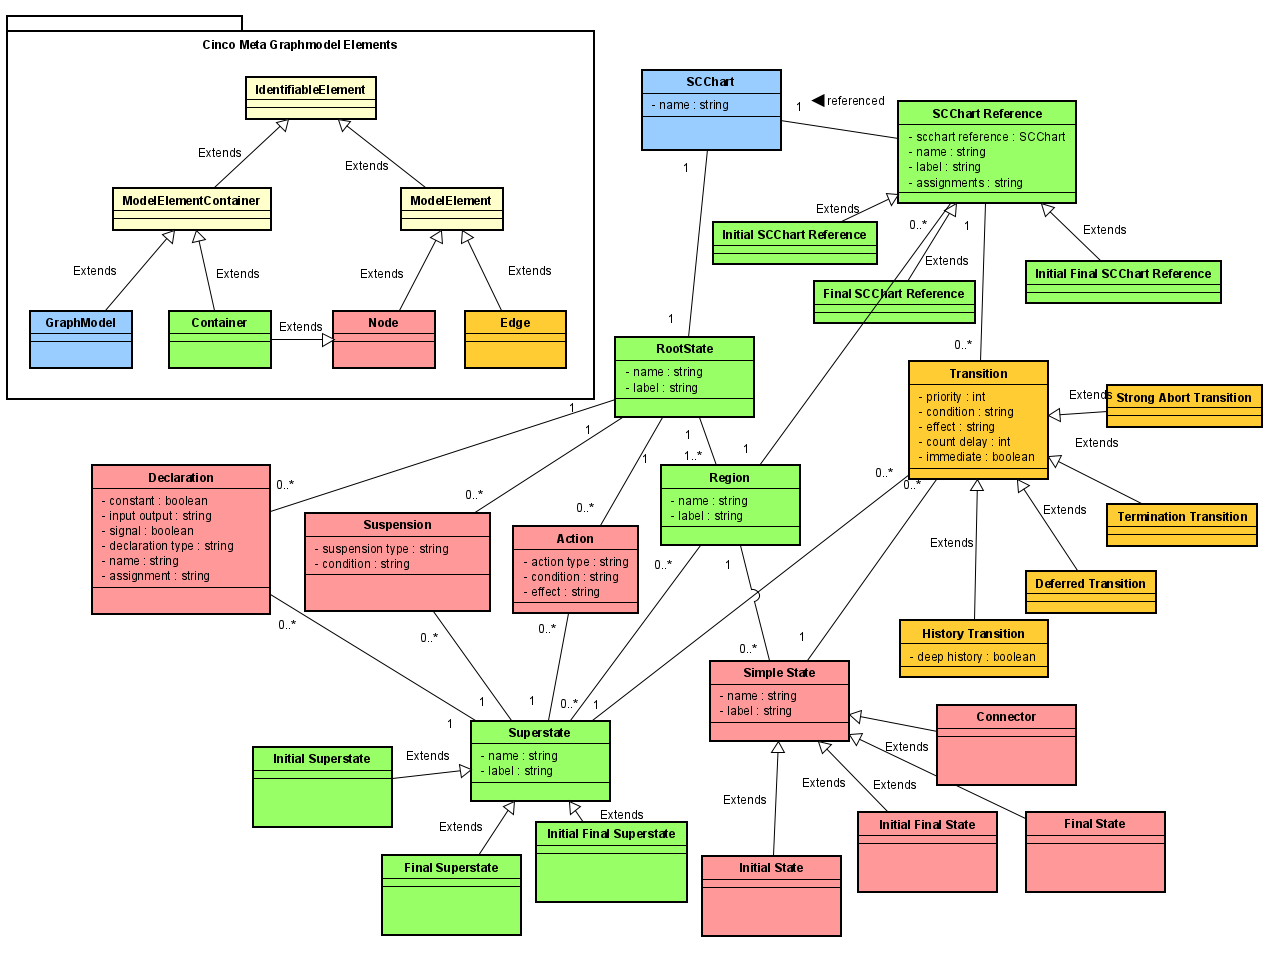
\includegraphics[width=1.0\textwidth]{bilder/MappingModelTransformation.png}
\caption{Mapping of \textsc{Cinco}'s meta graph model elements to the designed data structure for the SCCharts editor}
\label{fig:MappingModelTransformation}
\end{figure} 

\subsection{Implementation of the Meta Graph Language}
With the mapping as a basis, the realisation of the MGL can now begin. All components of the data structure are now implemented with the corresponding \textsc{Cinco}'s meta graph model type. In this section, only one representative for each meta graph model type is considered in more detail, as the implementation for the same types is similar. For the entire implementation of the SCChart MGL, see Appendix \ref{SCChart_MGL}.

\subsubsection{Graph Model}
In Listing \ref{graphmodel_MGL} is the implemented graph model of which there is only one in each MGL. After the keyword \textit{graphModel} the name of the component is given. In this case it is \textit{SCChart}. Then \textit{diagramExtension} is set in each graph model. This determines which file format the created graph model has. Here it is \textit{*.scchart}. \textit{ContainableElements} specifies which components SCChart graph model can contain. The data structure indicates that SCChart model has only one root state. Limits for the number of components can be realised in the MGL using square brackets. In addition, attributes can be defined in graph model, which is done here with name.
\lstinputlisting[frame=single,label=graphmodel_MGL,caption=The SCChart graph model implementation from the SCChart MGL,firstnumber=20,firstline=20, lastline=24]{Code/SCChart.mgl}

\subsubsection{Container}
Superstate was selected here as a representative for a component of the type container. The implementation can be seen in Listing \ref{SuperState_MGL}. All components except the graph model have a style, which is shown here with \textit{style} followed by the name of the style defined in the SGL. The string is an Xtext expression that ensures that if the label of Superstate is set, the label is passed along, otherwise the name. This allows the label for the component to be displayed in the editor if it is specified. Subsequently, in container, as with graph model, \textit{containableElements} can be used to determine which components superstate can contain. According to the data structure for superstate these are regions, declarations, actions, suspensions. \textit{IncomingEdges} and \textit{outgoingEdges} define which transitions can enter and exit. If these are not specified, no transitions can enter or exit. For Superstate, these are all transitions. This could actually be realised with '*', for all edges. However, since an abstract transition is defined in the MGL for the implementation and this should not be included in the model, all transitions must be entered here individually. Finally, the attributes for name and label are defined. For containers, nodes and edges, a class can be extended as usual in programming using the keyword \textit{extends}. In the MGL, the defined properties of the superclass are inherited. In this way, initial superstate, final superstate and initial final superstate are realised, whereby a style must still be specified here.
\lstinputlisting[frame=single,label=SuperState_MGL,caption=The superstate container implementation from the SCChart MGL,firstnumber=62,firstline=62, lastline=69]{Code/SCChart.mgl}

\subsubsection{Node}
In Listing \ref{graphmodel_MGL} the simple state component is shown as a representation for the type node. Nodes have similar properties to containers, except that they cannot contain elements. After the style is referenced, \textit{incomingEdges} and \textit{outgoingEdges} can be set, which are fewer compared to superstates. Although this is not directly evident from the data structure, it makes sense when considering the functions that some transitions have when entering or exiting a state. Since simple states have no internal behaviour, such transitions have no effect on them and would therefore be rather confusing. For this reason, the deferred and history transitions are missing from the incoming edges, and the strong abort and termination transitions are missing from the outgoing edges. Subsequently, attributes can be specified, in this case the name, which is already initialised, and the label. Initialising name with \textit{<set name>}, which has already been done for superstates, is to ensure later that the user gives the state a unique name.
\lstinputlisting[frame=single,label=SimpleState_MGL,caption=The simple state node implementation from the SCChart MGL,firstnumber=132,firstline=132, lastline=138]{Code/SCChart.mgl}

\subsubsection{Edge}
To better distinguish (normal) transition from other transition types, the superclass abstract transition was added, from which all twelve transition types inherit. Listing \ref{DeferredHistoryTransition_MGL} shows the implementation of the deferred history transition. The string contained in the referenced style is an Xtext expression with the function that the label of the edge has the format '[priority:] [[count delay] condition] [/ effect]'. Only the attributes of the label that have been set are displayed within the label. A second string is given for history transitions that is used for displaying deep history. Besides style, only attributes for edges can be defined.
\lstinputlisting[frame=single,label=DeferredHistoryTransition_MGL,caption=The deferred history transition edge implementation from the SCChart MGL,firstnumber=280,firstline=280, lastline=287]{Code/SCChart.mgl}

\subsubsection{Prime Viewer Meta Plug-In}
Listing \ref{PrimeViewer_MGL} shows the Prime Viewer plug-in. It is used to implement the reference in the data structure from the SCChartReference to an SCChart model. This must be activated before the graph model with the annotation \textit{@primeviewer}. Afterwards the annotation \textit{@pvFileExtension(...)} can be used to search for files of this format which contain the referenced model element. In this case the file extension is \textit{scchart} and the model element is SCChart. This is then assigned to \textit{reference}, which basically behaves like an attribute and contains all the information of the referenced SCChart.
\lstinputlisting[frame=single,label=PrimeViewer_MGL,caption=The Prime Viewer meta plug-in for SCChart reference,firstnumber=166,firstline=166, lastline=178]{Code/SCChart.mgl}

\subsection{Implementation of the Style Graph Language}
The visual appearance of the components from the MGL is defined in the MSL. In node styles, the visual representation of components of the type node or container can be defined and in edge style for components of the type edge. In this section, only one representative each of the node style and the edge style will be examined in more detail, as the implementation process of these styles is highly repetitive. For the entire implementation of the SCChart SGL, see Appendix \ref{SCChart_SGL}. In general, it is tried to stay as close as possible to the original syntax and visual representation of the SCCharts language with the given graphical elements and the settings of the appearance of the SGL.

\subsubsection{NodeStyle}
In node style, any number of container shapes, such as rounded rectangle or ellipse, or shapes such as text or polylines, can be defined. Container shapes can also contain other container shapes and shapes. Listing \ref{initialFinalSuperStateStyle_SGL} shows the node style of the component initial final superstate. The number in the bracket after the name determines the number of string parameters that must be provided by the components of the MGL. The name or label of the initial final superstate from the MGL is passed here. Then a container shape is implemented with \textit{roundedRectangle} and its appearance is determined with \textit{initialFinalStateOuterCircle}. In this case, it is a little wider line to indicate the initial feature. Then the size is set with \textit{size()} and the rounded corners with \textit{corner()}. In addition, another inner rounded rectangle is defined whose appearance determines the fore and background colour. With \textit{position} the location of the inner rectangle can be set in the outer rectangle. The size and the rounded corners can be adjusted as for the outer rectangle. Thus, the component has a double border indicating the final feature. In the inner rectangle, a text is defined that receives the parameter string and displays it in the middle at the top of the inner rectangle. The visual representation in the editor of the initial final superstate is shown in Fig. \ref{fig:SGL_Elements} left.
\lstinputlisting[frame=single,label=initialFinalSuperStateStyle_SGL,caption=The initial final superstate style implementation from the SCChart SGL,firstnumber=163,firstline=163, lastline=180]{Code/SCChart.style}

\subsubsection{EdgeStyle}
In edge styles, the appearance of the connecting line and the decorators can be defined. As with node style, a string must be given as argument for termination transition, as shown in Listing \ref{terminationTransitionStyle_SGL}. The appearance provider is used for every transition type to change the line of the edge from solid to dashed on runtime if the transition is immediate, i.e. the boolean \textit{immediate} is true. In this way, it is not necessary to define an equivalent immediate transition type in the MGL for each transition type. Furthermore, termination transitions are also displayed as dashed transitions if they are unconditional. The referenced class of the Appearance Provider is an Xtend class for each transition type, in which the function when to change the appearance is implemented. After that, the default appearance is set. In addition, decorators are defined that lie on or at the line. These can have predefined shapes like the first decorator (arrow). The location also specifies the relative position of the decorator to the edge. An appearance can also be specified for each decorator. The second decorator is a self-defined green triangle at the beginning of the transition, which indicates the termination of the source state. The last decorator displays the text, i.e. the label of the edge, which includes priority, condition, count delay and effect. This is displayed in the centre and can be moved because of the \textit{movable} keyword. The representation of the termination transition in the editor is shown right in Fig. \ref{fig:SGL_Elements}
\lstinputlisting[frame=single,label=terminationTransitionStyle_SGL,caption=The termination transition style implementation from the SCChart SGL,firstnumber=347,firstline=347, lastline=369]{Code/SCChart.style}

\begin{figure}[h!]
\centering
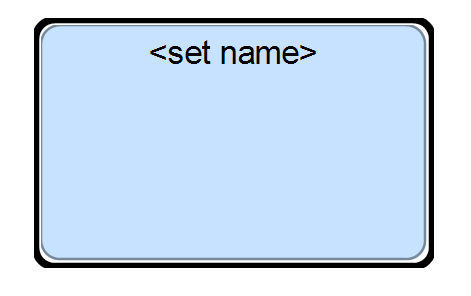
\includegraphics[width=0.5\textwidth]{bilder/SGL_InitFinSuper_Shape.png}
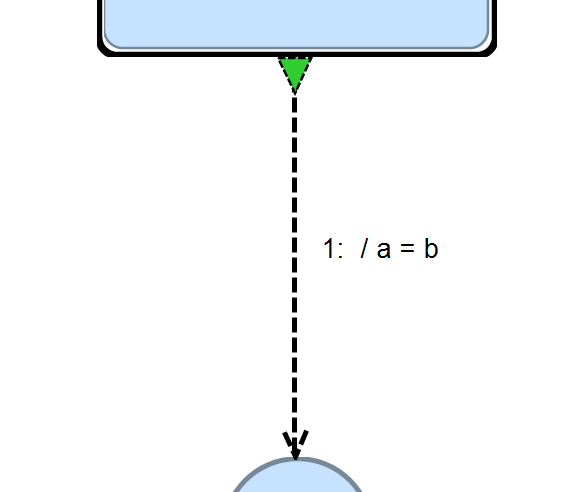
\includegraphics[width=0.4\textwidth]{bilder/SGL_TermTran_Shape.png}
\caption{Visual representation of the initial final superstate (left) and the termination transition (right) in the editor}
\label{fig:SGL_Elements}
\end{figure} 

\section{User Interface and Model Validation}
Although it is already possible to create SCChart models with the implementation of MGL and SGL, the editor, in its current state, would not provide a good user experience. The issue is illustrated in Fig. \ref{fig:Bad_User-Interface}. All components of the type container and node are listed under the \textit{node} tab on the right-hand side. A model with several components has been created in the middle. When components are created by drag and drop, they are created at the location where they are dropped with the specified size defined in the SGL. This may mean that the component created is too large for the container or that the component should not be displayed in this position. This can lead to the creation of confusing diagrams. It is also tedious to have to manually adjust the nodes and containers every time when creating new components or deleting old ones. The KIELER SCChart tool suit (Sec. \ref{Kieler}) has an automatic layout which, when designing SCCharts after changes to the SCT, automatically arranges the model appropriately. Within the scope of this bachelor thesis it is not possible to realise such a comprehensive layout program. But with the meta plug-ins from \textsc{Cinco}, the usability of the editor can be improved with little effort. Therefore, it would be useful if declarations, suspensions and actions were arranged in a superstate or root state directly in the upper area when they are created and the remaining declarations, suspensions and actions are rearranged when they are deleted in order to close any gaps that occur. The same applies to regions. These are to be integrated next to other regions with the same distance to them or also to the border when they are created. In addition, not all functions such as resizing, deleting or moving should be possible for all components, as e.g. simple states should have a constant size. In the next sections, meta plug-ins and their implementation are presented, which improve the user-friendliness of the editor.

\begin{figure}[h!]
\centering
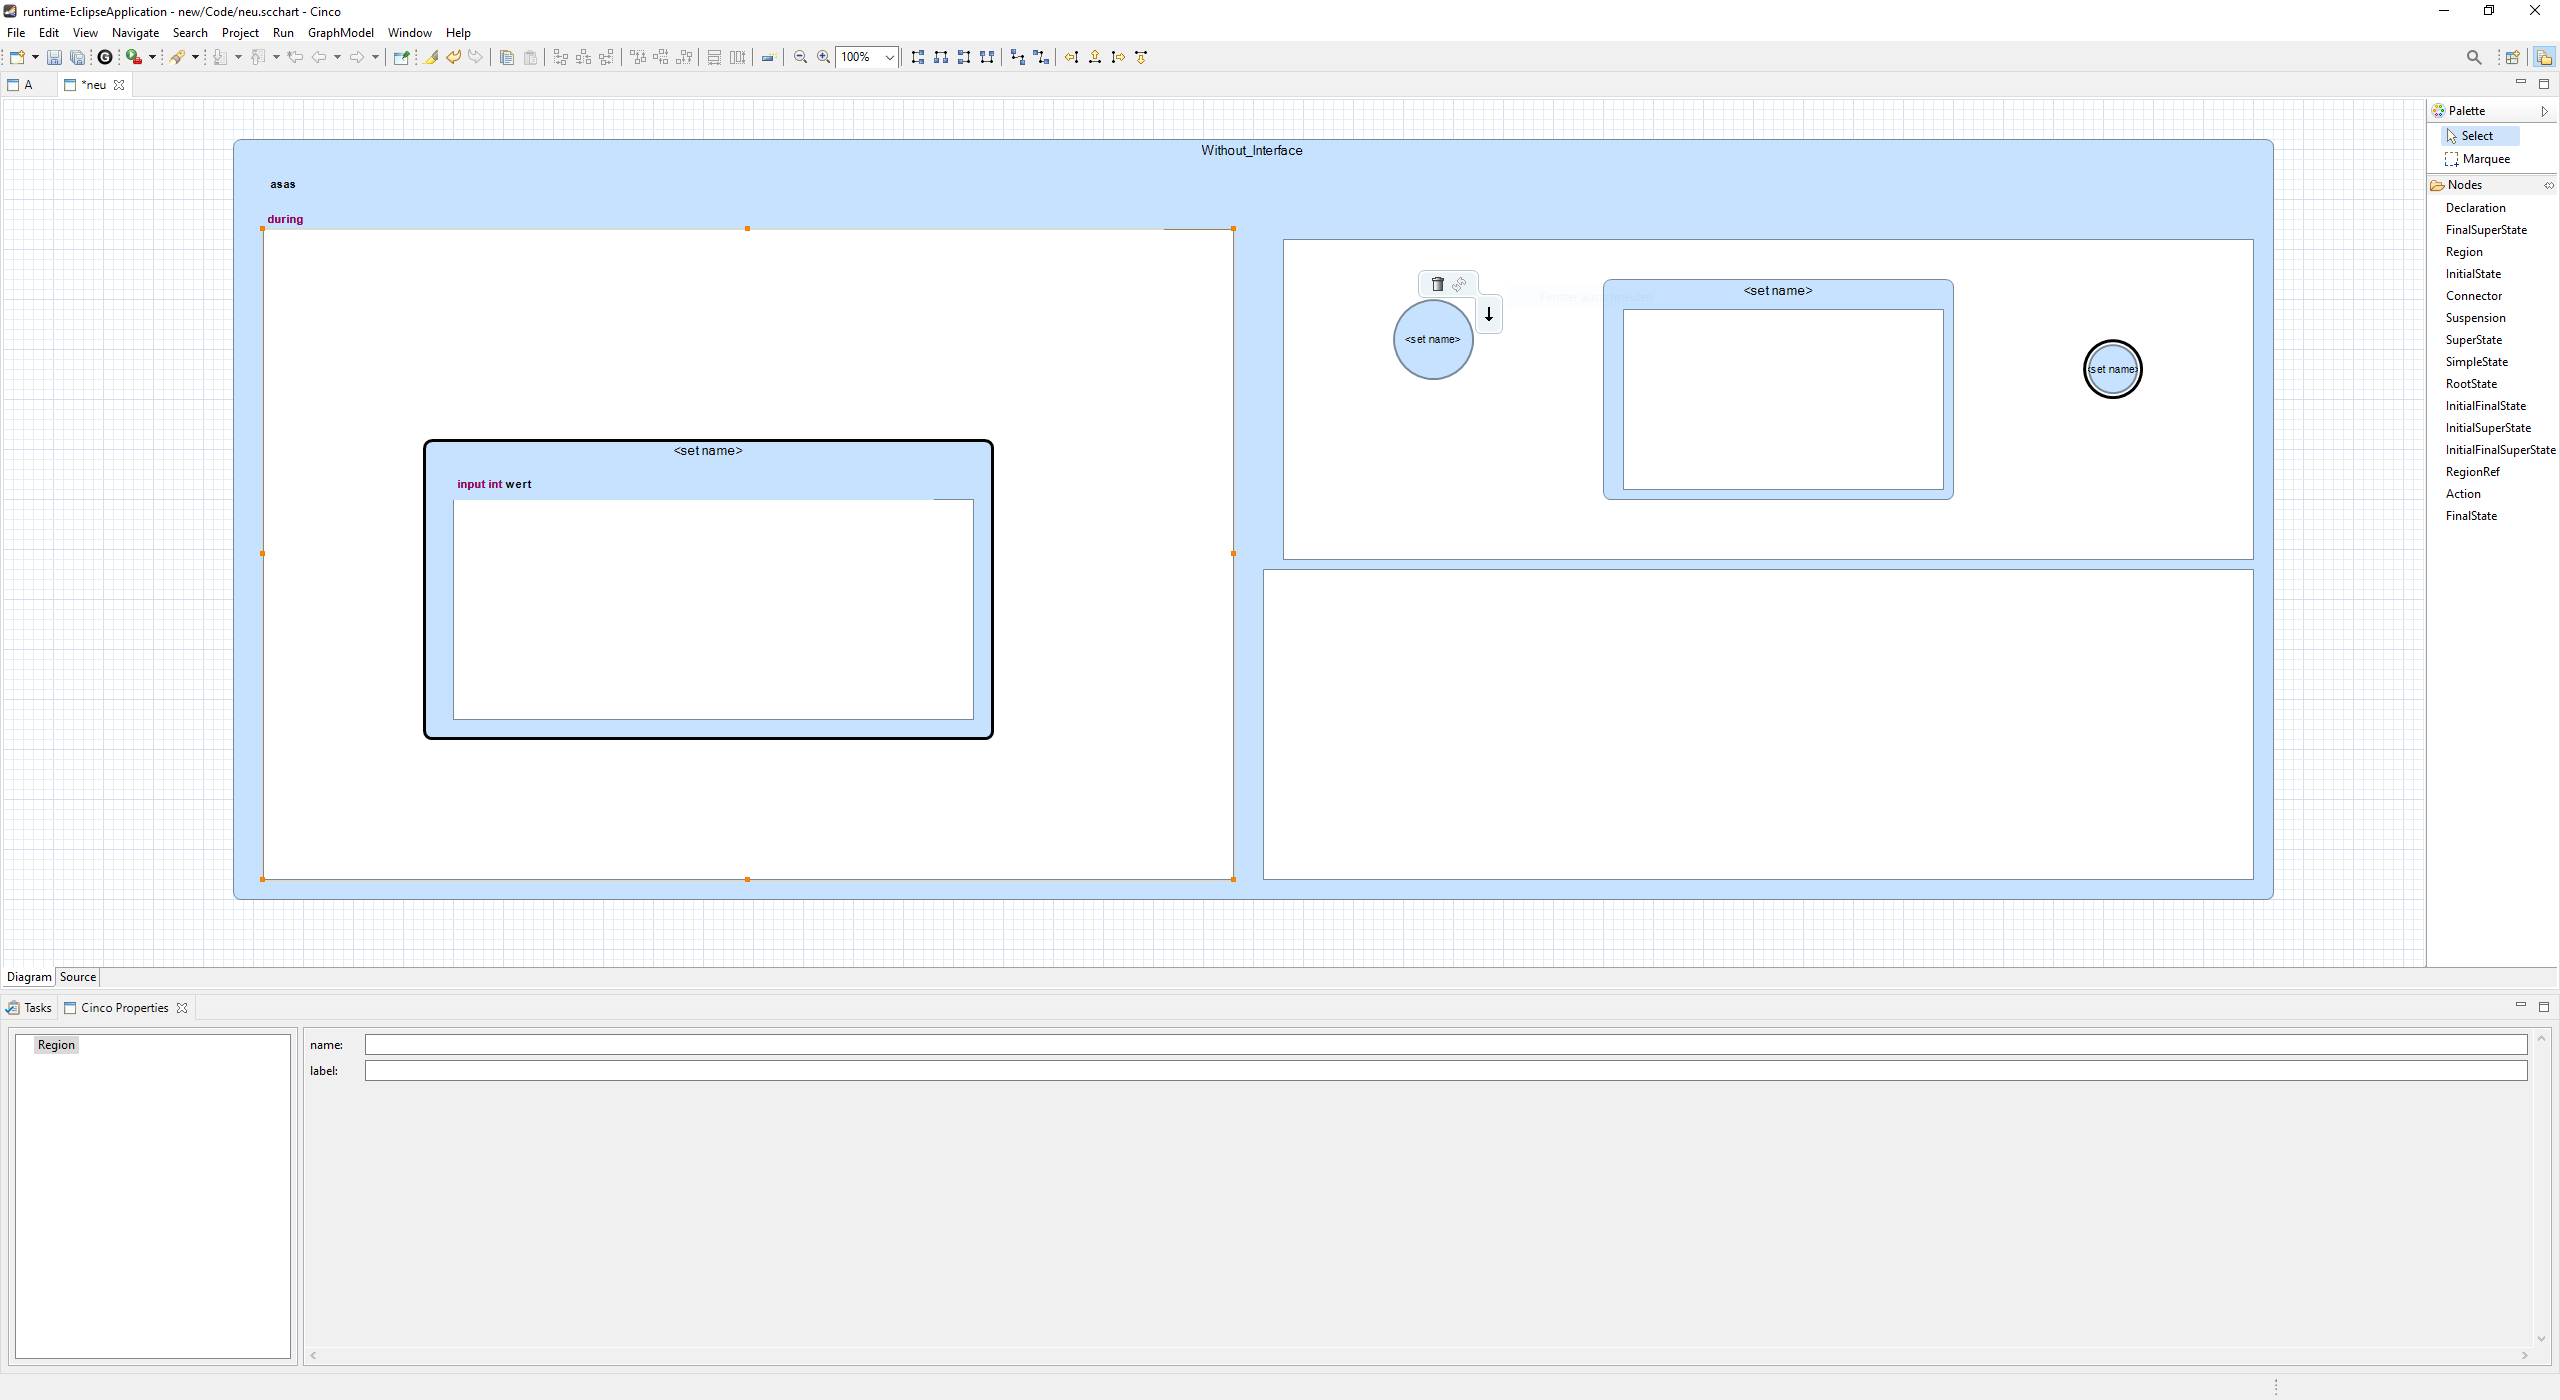
\includegraphics[width=1.0\textwidth]{bilder/Bad_User-Interface.png}
\caption{The SCCharts editor without plug-ins}
\label{fig:Bad_User-Interface}
\end{figure} 

\subsection{Event API}
The Event API can be used to react to various events in the editor. These events can be, for example, the creation or moving of a component. The Event API can be activated for a component in the MGL by annotation and can be applied to all component types. In the corresponding event class of the component, the functionality can be implemented for an event.

For the SCChart graph model, the Event API is used to automatically create a root state with a region after creation. This is because every SCChart has a root state. Furthermore, for superstates and the root state, regions, declarations, suspensions and actions are automatically adjusted to the new size of the superstate or root state after a change in size. 


In order for declarations, suspensions and actions to be listed in the upper left corner of their associated states, within the Event API a function is implemented for each component, which is called when the respective component is created. Listing \ref{actionPostCreate} shows, as an example, a part of the code implemented for the \textit{postCreate} event of action. For the arrangement of the elements in the respective states, these must be accessed. Since the superstate or root state cannot be accessed directly as the respective instance, the SCChart model is called via the method \textit{rootElement} and then the state that contains the created action node is identified via a tree-like search. To identify the state containing the created action node, a random UUID is assigned via the Java UUID (Universally Unique Identifier) class when the action node is created (line 34). This requires an additional attribute to be defined in the MGL for actions. To make it invisible to the user of the editor, it is hidden in the editor with the annotation \textit{@propertiesViewHidden}. The algorithm first iterates the root state and searches in the list of actions (if not null) for an element with the UUID of the created element (lines 36-38). If the action node with the UUID is found in the root state, action nodes are reordered with the created action (lines 39-51). To do this, the number of declarations and suspensions are first determined (lines 39-45) in order to be able to place the action nodes below them. Then a check is made to see if a region has been obscured by the placement of the action node. If this is the case, the region is reduced accordingly (lines 53-60). If the created action is not in the root state, the superstates in the regions of the root state are searched for the element (lines 65-73). The method \textit{postCreateAction()} (line 69) is similar in structure to \textit{postCreate()} (line 33). The only difference is that the action node created is searched in a superstate and instead in a root state. This method is also recursive, i.e. in each superstate in which the element was not found and in whose regions there are still superstates, the function is called again for the superstates contained. Similar methods were used for post creations of declarations or suspensions. And similar procedures are also implemented for post deletion of corresponding components, which ensure that no gaps exist within declarations suspensions and actions, and regions resize accordingly when space is freed up at the top of the state. For the entire implementation of the Xtend ActionEvent class, see Appendix \ref{ActionEvent_Xtend}.
\lstinputlisting[language=xtend,frame=single,label=actionPostCreate,caption=Part of the implementation in Xtend for the postCreate method of the action event class,firstnumber=33,firstline=33,lastline=74]{Code/ActionEvent.xtend}

The Event API is also used to arrange regions when they are created in a state. Again, the root state or superstate in which the region is created must be accessed, so a similar search algorithm is used as for actions. For this, region also receives a hidden UUID attribute in the MGL. If state containing the created region is found, the region next to it (if exists) is halved (minus the distance between them) and the region created is placed on the area that becomes free with the same size as the halved region. For better understanding an example for this is shown in \ref{fig:Event_region}. The arrows indicate on which side the new region was created and what the superstate looks like after the regions have been arranged. If a region is created between two regions, the left or upper region is first used to create the new region. If there is no region in the state, the created region will have the entire size of the state minus the distance to the borders. During the implementation, cases occurred where the region was simply placed but not arranged, which could lead to the creation of incorrect models. For this case, the algorithm was extended so that the region is deleted automatically if it is not arranged, so that the user can try to create a new region again. For the post delete function of regions, the create function is basically reversed. Again, the state that contained the deleted region is searched first, and then a neighbouring region of similar size to the deleted region is searched for. In this way, the region takes up the area of the deleted region without covering other regions or leaving free areas in the state. With these simple methods of the event classes, components can be dynamically created, deleted and resized.
\begin{figure}[h!]
\centering
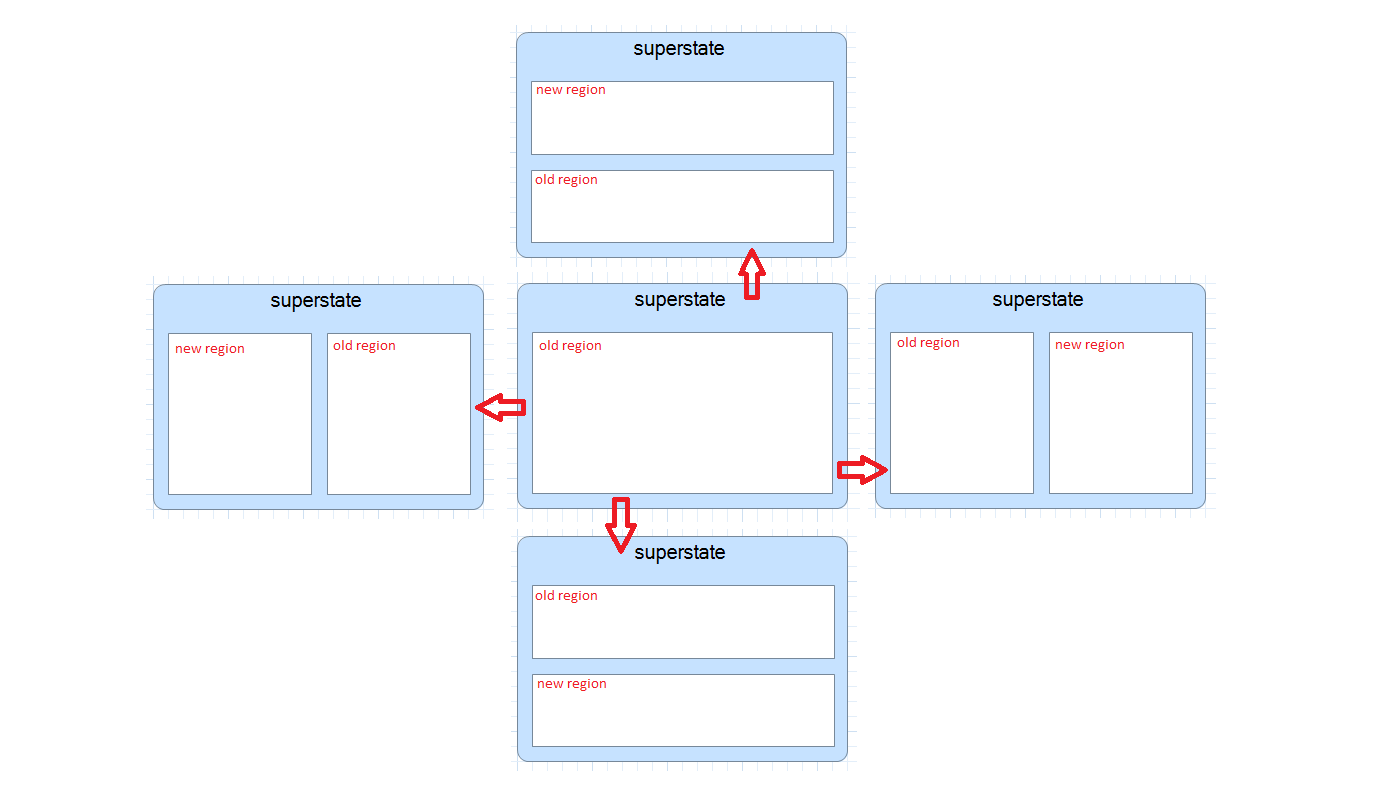
\includegraphics[width=1.0\textwidth]{bilder/Event_region.png}
\caption{Ordering mechanism of created regions in states}
\label{fig:Event_region}
\end{figure} 

\subsection{Palette, Disable, Possible Value Provider}
Besides the Event API, which can be used to implement many different functions, there are also smaller plug-ins that can be applied to improve the user interface. These are briefly presented below.

With the palette plug-in, containers and nodes can be grouped under their own term on the right-hand side of the editor, which improves clarity for the user. For example, superclasses can be combined with subclasses under the\textit{Superstates} tab. In addition, components can be hidden if no term is specified in the palette name. This is used for the root state, as it only exists once in SCChart and is created directly when an SCChart model is created via the Event API.

In the editor it is desirable that certain functions such as resize or move are not available for some components. Otherwise, the user can make changes to the model that are not intended. \textit{@disable} can be used for this purpose by disabling the functions move, select, create, resize and delete in the editor for certain components. Thus, resize is disabled for simple states and their subclasses, as their size should be adjustable. Furthermore, move and resize are disabled for region and declarations, suspensions and actions, as their arrangement and resizing is controlled by the Event API. In addition, delete has been disabled for root state, as the user should not be able to delete it.

The Possible Value Provider plug-in can be used to specify certain values for attributes of components to ensure that users cannot make invalid entries. This is used in declarations, actions and suspensions, e.g. to define the type. In addition, the possible selection of the priority of outgoing transitions for states is defined, whereby the selection option is bound to the number of outgoing edges.

\subsection{Model Compare and Merge Framework}
The Model Compare and Merge (MCaM) framework can be used to perform validations during model creation in the editor. To do this, it is activated with \textit{@mcam("check")} in the MGL. Subsequently, with \textit{@mcam\_checkmodule()} the classes in which the validations are implemented are registered in the MGL. For a better overview during implementation, it makes sense to create a separate check module for each class or superclass of the MGL.

Thus, a priority check for transitions is implemented, which checks whether the outgoing edges of each node and container of the model have a valid priority. A further function checks whether the source and target elements of a transition are in the same region. Another example is the check for regions that must always have exactly one initial state, initial superstate or initial SCChart reference. Other, but certainly not all, checks are implemented.


\section{Implementation of the Code Generator}
After the user interface has been adapted and validation functions realised, models can now be created. To be able to convert these models into C or Java code, a code generator must be implemented.

The Generatable meta plug-in of \textsc{Cinco} is a tool, that utilises template expressions of Xtend and can be used to attempt to translate SCChart models into Java or C code. However, this would be elaborately, as it is not so easy to translate the features of the SCCharts language into corresponding Java and C code artefacts. A simpler method is to use the KIELER Compiler CLI from Sect. \ref{Kieler}, which can generate C or Java code from SCT. This means that the components of the model would have to be converted into SCT format using the code generator and then passed to the KIELER Compiler CLI.
In Fig. \ref{fig:SCChartsCheatSheetMod} Core SCCharts and Extended SCCharts are shown with SCT translations for each component in the margin. Most of the SCT translations are already illustrated here. The only missing component are the SCChart references, which need to be called at the beginning of an SCT file with an import statement, and further defined in a second call. 

\begin{figure}[h!]
\centering
\includegraphics[width=1.0\textwidth]{bilder/SCChartsCheatSheetMod.png}
\caption{Core- and Extended SCCharts with SCT annotation~\cite{.06.05.2022}.}
\label{fig:SCChartsCheatSheetMod}
\end{figure} 

For the model to text transformation, a function is defined for each component in the code generator plug-in, as shown in Fig. \ref{fig:CodeGenClasses}. This function is responsible for placing keywords and attributes of its component at the appropriate location in the SCT file. For components of type container, the containing components are invoked along with their defined functions.

To show what such a function looks like, Listing \ref{CodeGenTemp} shows the template function that is used to translate the root state of the SCChart graph model into SCT. The generation of the other components of the SCChart model originates from here. ''' in line 60 indicates that this is a template expression, i.e. text indentation is taken into account outside the french prefixes.  In lines 61-63, the imports for possible referenced SCCharts are converted. Then follows the formatting for the root state with \textit{scchart} as the keyword and, separately, the name of the root state. Within the curly brackets, the declarations, suspensions, actions, and regions contained in the root state in this order are then called with the corresponding functions (lines 65-84). 
\lstset{literate=
  {á}{{\'a}}1 {é}{{\'e}}1 {í}{{\'i}}1 {ó}{{\'o}}1 {ú}{{\'u}}1
  {Á}{{\'A}}1 {É}{{\'E}}1 {Í}{{\'I}}1 {Ó}{{\'O}}1 {Ú}{{\'U}}1
  {à}{{\`a}}1 {è}{{\`e}}1 {ì}{{\`i}}1 {ò}{{\`o}}1 {ù}{{\`u}}1
  {À}{{\`A}}1 {È}{{\`E}}1 {Ì}{{\`I}}1 {Ò}{{\`O}}1 {Ù}{{\`U}}1
  {ä}{{\"a}}1 {ë}{{\"e}}1 {ï}{{\"i}}1 {ö}{{\"o}}1 {ü}{{\"u}}1
  {Ä}{{\"A}}1 {Ë}{{\"E}}1 {Ï}{{\"I}}1 {Ö}{{\"O}}1 {Ü}{{\"U}}1
  {â}{{\^a}}1 {ê}{{\^e}}1 {î}{{\^i}}1 {ô}{{\^o}}1 {û}{{\^u}}1
  {Â}{{\^A}}1 {Ê}{{\^E}}1 {Î}{{\^I}}1 {Ô}{{\^O}}1 {Û}{{\^U}}1
  {ã}{{\~a}}1 {ẽ}{{\~e}}1 {ĩ}{{\~i}}1 {õ}{{\~o}}1 {ũ}{{\~u}}1
  {Ã}{{\~A}}1 {Ẽ}{{\~E}}1 {Ĩ}{{\~I}}1 {Õ}{{\~O}}1 {Ũ}{{\~U}}1
  {œ}{{\oe}}1 {Œ}{{\OE}}1 {æ}{{\ae}}1 {Æ}{{\AE}}1 {ß}{{\ss}}1
  {ű}{{\H{u}}}1 {Ű}{{\H{U}}}1 {ő}{{\H{o}}}1 {Ő}{{\H{O}}}1
  {ç}{{\c c}}1 {Ç}{{\c C}}1 {ø}{{\o}}1 {Ø}{{\O}}1 {å}{{\r a}}1 {Å}{{\r A}}1
  {€}{{\euro}}1 {£}{{\pounds}}1 {«}{{\guillemotleft}}1
  {»}{{\guillemotright}}1 {ñ}{{\~n}}1 {Ñ}{{\~N}}1 {¿}{{?`}}1 {¡}{{!`}}1 
}
\lstinputlisting[language=xtend,frame=single,label=CodeGenTemp,caption=Template function of the SCChart code generator,firstnumber=60,firstline=60,lastline=86]{Code/CodeGenerator.xtend}

In SCT, priority is regulated so that transitions with the highest priority are placed directly after the source element, followed by transitions with the second-highest priority, and so on. For this purpose, an extra function, \textit{genEdgesOrder(...)}, is implemented that outputs the transitions for components with outgoing edges in the correct order after the component. The generated file with the file extension *.sctx is saved in the folder specified in the MGL in the workspace. 

In addition, a command line call with the method \textit{commandLineParser} is implemented, that invokes the KIELER Compiler CLI and passes the generated file in SCT format along with instructions for the target language as parameters and target directory. The target directory is the folder in which the SCT file is located. The KIELER Compiler CLI offers different compilation variants for Java and C. It also offers the possibility to convert the SCT file into a diagram, which can be useful for validating the created model with the editor. In total, there are seven different types of compilation. For this reason, another attribute is defined in the MGL for root state, which is used in the editor to select the target language of the code generator. The plug-in Possible Value Provider is used for this purpose. With this, the user can select one of the possible compilation types. This code generator is written for the Windows operating system, as it calls the \textit{cmd.exe}. However, it can easily be implemented for other operating systems by calling the appropriate terminal application.

\begin{figure}[h!]
\centering
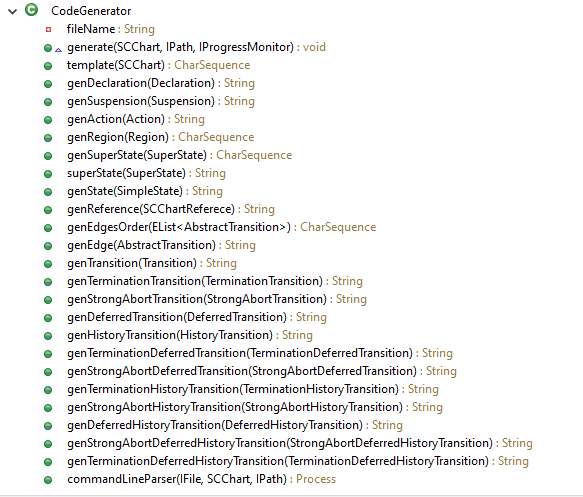
\includegraphics[width=1.0\textwidth]{bilder/CodeGenClasses.png}
\caption{Methods of the implemented Xtend class from code generator plug-in}
\label{fig:CodeGenClasses}
\end{figure} 

